\documentclass[12pt,a4paper]{article}

\usepackage[utf8]{inputenc}
\usepackage[T1]{fontenc}
\usepackage[margin=2.5cm]{geometry}
\usepackage{enumitem}
\usepackage{fancyvrb}
\usepackage{booktabs}
\usepackage{longtable}
\usepackage{graphicx}
\usepackage[hidelinks]{hyperref}

\newcommand{\drawiolink}[2]{\href{run:diagrams/#1}{\texttt{#2}}}

\title{\textbf{Flower Supply}\\Servlet Application}
\author{Student: \textit{Vararean Diana-Lorena}\\Group: \textit{244}}

\begin{document}

\maketitle
\tableofcontents
\newpage

\section{Introduction}

Flower Supply is a small supply application implemented with Jakarta Servlets. It models one flower shop that requests stock from one central warehouse.

The application consists of two independent Maven web projects. The Warehouse
service runs in Tomcat and owns the central stock, while the Shop service runs in Jetty and owns the local shop stock. The Shop communicates with the Warehouse through a synchronous HTTP/JSON request. A request is immediately approved or rejected and the Shop updates its local stock only after obtaining an approval. This implementation relies on Tomcat and Jetty as the servlet containers for deployment and execution. 

\section{Architecture}

\begin{figure}[htbp]
    \centering
    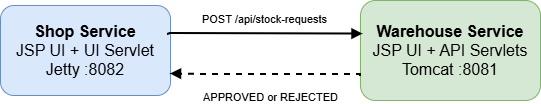
\includegraphics[width=0.8\textwidth]{diagrams/servlets1.png}
    \caption{System Architecture Overview}
    \label{fig:architecture}
\end{figure}

Each service is packaged as a separate WAR file. The services do not share
Java classes or in-memory state. The Warehouse exposes the only public JSON
API. The Shop exposes UI pages only.

\section{Technologies and System Calls}

\begin{itemize}[leftmargin=*]
    \item Java 21 and Maven WAR packaging;
    \item Jakarta Servlet API 6.0;
    \item Tomcat for the Warehouse and Jetty for the Shop;
    \item JSP and JSTL for server-rendered user interfaces;
    \item Jackson for JSON serialization and deserialization;
    \item \texttt{java.net.http.HttpClient} for the synchronous service call;
    \item \texttt{ConcurrentHashMap} for in-memory stock storage;
    \item HTTP system calls through the Java HTTP client and command-line
    \texttt{curl} during verification.
\end{itemize}

No data is written at runtime. At startup, each application reads its own CSV
file from the classpath. A restart therefore resets the stock to the CSV
values.

\section{Data Model and Storage}

The \texttt{Flower} object has three properties:
\begin{itemize}
    \item \texttt{flowerId: String}
    \item \texttt{name: String}
    \item \texttt{quantity: int}
\end{itemize}

The CSV format is the following:
\begin{Verbatim}
flowerId,name,quantity
rose-red,Red Rose,200
\end{Verbatim}

The Warehouse and Shop each have a separate \texttt{StockStore} singleton.
The Warehouse uses an atomic synchronized approval operation. It checks
existence and available quantity and decrements the flower in the same
critical section. The Shop uses synchronized increase and decrease operations
so that a local stock update cannot be partially applied.

\section{Warehouse Service}

\paragraph{Objects and method prototypes.}

\begin{longtable}{p{0.34\textwidth}p{0.58\textwidth}}
\toprule
\textbf{Object} & \textbf{Public constructors and methods}\\
\midrule
\endhead
\texttt{Flower} &
\texttt{Flower()}\\
& \texttt{Flower(String flowerId, String name, int quantity)}\\
& \texttt{String getFlowerId()}\\
& \texttt{String getName()}\\
& \texttt{int getQuantity()}\\
& setters for the three properties\\[2pt]
\texttt{StockStore} &
\texttt{static StockStore getInstance()}\\
& \texttt{void loadFromCsv(InputStream input) throws IOException}\\
& \texttt{List<Flower> findAll()}\\
& \texttt{boolean approveRequest(String flowerId, int requestedQuantity)}\\[2pt]
\texttt{WarehouseStartupListener} &
\texttt{void contextInitialized(ServletContextEvent event)}\\[2pt]
\texttt{StockServlet} &
\texttt{void doGet(HttpServletRequest request, HttpServletResponse response)
throws IOException}\\[2pt]
\texttt{StockRequestServlet} &
\texttt{void doPost(HttpServletRequest request, HttpServletResponse response)
throws IOException}\\[2pt]
\texttt{WarehouseUiServlet} &
\texttt{void doGet(HttpServletRequest request, HttpServletResponse response)
throws ServletException, IOException}\\
\bottomrule
\end{longtable}

\paragraph{API contract.}

\begin{longtable}{p{0.33\textwidth}p{0.68\textwidth}}
\toprule
\textbf{Request} & \textbf{Processing and output}\\
\midrule
\texttt{GET /warehouse/api/stock} &
Returns HTTP 200 and a JSON array containing the current warehouse stock.\\
\texttt{POST /warehouse/api/stock-requests} &
Receives \texttt{\{"flowerId": String, "quantity": int\}}. For a valid
request, returns HTTP 200 and either \texttt{\{"status":"APPROVED"\}} or
\texttt{\{"status":"REJECTED"\}}.\\
Invalid request &
Malformed JSON, missing fields, empty flower identifier, or
\texttt{quantity <= 0} returns HTTP 400.\\
\bottomrule
\end{longtable}

\section{Shop Service}

\paragraph{Objects and method prototypes.}

\begin{longtable}{p{0.34\textwidth}p{0.58\textwidth}}
\toprule
\textbf{Object} & \textbf{Public constructors and methods}\\
\midrule
\endhead
\texttt{StockStore} &
\texttt{static StockStore getInstance()}\\
& \texttt{void loadFromCsv(InputStream input) throws IOException}\\
& \texttt{List<Flower> findAll()}\\
& \texttt{boolean increase(String flowerId, int quantity)}\\
& \texttt{boolean decrease(String flowerId, int quantity)}\\[2pt]
\texttt{WarehouseClient} &
\texttt{StockRequestResult requestStock(String flowerId, int quantity)}\\[2pt]
\texttt{StockRequestResult} &
\texttt{StockRequestResult(Status status, String message)}\\
& \texttt{Status status()}\\
& \texttt{String message()}\\[2pt]
\texttt{ShopStartupListener} &
\texttt{void contextInitialized(ServletContextEvent event)}\\[2pt]
\texttt{ShopServlet} &
\texttt{void doGet(HttpServletRequest request, HttpServletResponse response)
throws ServletException, IOException}\\
& \texttt{void doPost(HttpServletRequest request, HttpServletResponse response)
throws ServletException, IOException}\\
\bottomrule
\end{longtable}

\paragraph{User interface.}

The Shop JSP displays the current stock in a table. Flowers with quantity
strictly below 10 receive a red visual highlight and a \texttt{LOW} label.
The page provides two forms:

\begin{itemize}
    \item a warehouse request form containing a flower and a positive quantity;
    \item a local decrease form simulating a sale.
\end{itemize}


The Shop uses a two-second connection timeout and a five-second request
timeout. If the Warehouse cannot be reached, the page shows
\texttt{Warehouse is unavailable} and does not change local stock. No retry is
performed.

\section{Processing Sequence}

The following processing diagram documents the main path from a user submission to the final page.

\begin{figure}[htbp]
    \centering
    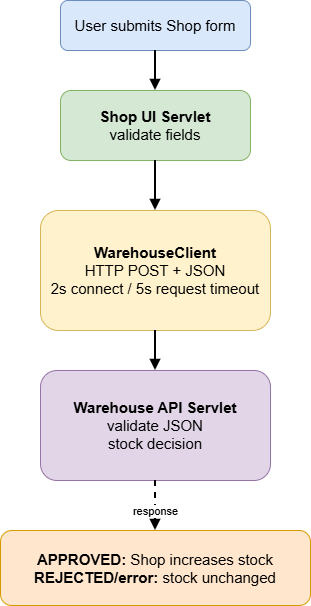
\includegraphics[width=0.4\textwidth]{diagrams/servlets2.png}
    \caption{Synchronous request processing}
    \label{fig:processing}
\end{figure}

The following steps outline the synchronous request processing in detail:

\begin{enumerate}
\item The user submits the Shop request form.
\item \texttt{ShopServlet} validates the form values.
\item \texttt{WarehouseClient} sends an HTTP POST with JSON.
\item \texttt{StockRequestServlet} validates the JSON and atomically checks the available Warehouse stock.
\item The Warehouse processes the request and returns a decision:
\begin{itemize}
\item \textbf{Approved:} If stock is sufficient, the Warehouse decrements its inventory and returns \texttt{APPROVED}. The Shop then increases its local quantity.
\item \textbf{Rejected:} If the flower is unknown or stock is insufficient, the Warehouse returns \texttt{REJECTED}. The Shop's local stock remains unchanged.
\end{itemize}
\item The Shop renders the updated page to the user.
\end{enumerate}

If the HTTP call times out, the Warehouse cannot be reached, or the response is invalid, the client reports an error and the local Shop stock remains unchanged.

\section{Deployment and Examples}

The deployment is manual, and the project produces two independent WAR files. The Warehouse WAR is copied to the Tomcat \texttt{webapps} directory and the Shop WAR is copied to the configured Jetty deployment directory.
The \texttt{warehouse.war} produces the \texttt{/warehouse} context and
\texttt{shop.war} produces the \texttt{/shop} context.

\paragraph{Build and deployment sequence.}

\begin{enumerate}
    \item Verify that Java 21, Maven, Tomcat, and Jetty are installed.
    \item Run the unit tests and build each WAR:
\begin{Verbatim}
cd warehouse-service && mvn clean test package
cd ../shop-service && mvn clean test package
\end{Verbatim}
    \item Copy \texttt{warehouse-service/target/warehouse.war} to the
    Tomcat deployment directory.
    \item Copy \texttt{shop-service/target/shop.war} to the Jetty deployment
    directory.
    \item Start both application servers and wait for their deployment
    scanners to load the WAR files.
    \item Verify the UI and the Warehouse JSON endpoints.
\end{enumerate}

\paragraph{Project lifecycle script.}

\texttt{run.sh} is located in the project root and delegates server lifecycle
operations to the existing scripts in the parent \texttt{servers} directory.
It calculates paths relative to its own location, so it can be called from
any current directory. The available commands are:

\begin{longtable}{p{0.25\textwidth}p{0.66\textwidth}}
\toprule
\textbf{Command} & \textbf{Operation}\\
\midrule
\texttt{./run.sh build} & Run Maven tests and create both WAR files.\\
\texttt{./run.sh deploy} & Build, copy both WAR files, restart both servers,
and wait until both HTTP URLs respond.\\
\texttt{./run.sh start} & Start Tomcat and Jetty, then wait for readiness.\\
\texttt{./run.sh stop} & Stop Jetty and Tomcat using their stop scripts.\\
\texttt{./run.sh restart} & Stop and start both application servers.\\
\texttt{./run.sh status} & Probe the two UI URLs and report running or stopped.\\
\texttt{./run.sh test} & Run the integration script against both deployed
applications.\\
\bottomrule
\end{longtable}

The Warehouse API can be tested with:

\begin{Verbatim}
curl -X POST http://localhost:8081/warehouse/api/stock-requests \
  -H 'Content-Type: application/json' \
  -d '{"flowerId":"rose-red","quantity":50}'
\end{Verbatim}

The expected successful response is:

\begin{Verbatim}
{"status":"APPROVED"}
\end{Verbatim}

\section{Testing}

Unit tests cover CSV loading, valid and invalid Warehouse requests, stock
decrease and increase operations, and the strict low-stock boundary: quantity
9 is low stock while quantity 10 is not. Integration tests cover both
UIs, the approved and rejected flows, malformed requests, unavailable
Warehouse behavior, simultaneous server execution, and reset after restart.

\section{Additional Solution}

The implemented solution uses synchronous HTTP/JSON because the assignment
requires an immediate decision. A message queue would decouple the services
and support asynchronous processing. A larger REST client layer could provide versioned API contracts,
but the current two-endpoint API is sufficient for one Shop and one
Warehouse.


\end{document}
